\documentclass[
	letterpaper
	12pt
]{template}
\usepackage{wrapfig}
\usepackage{apacite}
\usepackage{titling}
\usepackage{multicol}
\usepackage{caption}


\usepackage[font=footnotesize,labelfont=bf]{caption}

\setlength{\droptitle}{-10em}

\newcommand{\bref}[2]{\textbf{\hyperref[#1]{#2}}}

\title{Pendulum Project}

\author{Sebastien Psarianos}

\date{\today}



\begin{document}
\maketitle
\section{Introduction}
In this report, we analyze the simple damped pendulum model (\bref{eqn::oscillatorEqn}{Equation 1}) as applied to a real world pendulum moving in a 2D plane. By verifying the accuracy of certain predictions of the model and analyzing the effect of oscillation angles far outside the ``small angle approximations'', we aim to quantify the model's accuracy.

\subsection{Background}
The differential equation that describes a linear restoring force with a velocity proportional damping factor is given by:
\begin{equation}\label{eqn::oscillatorEqn}
		\ddot{x} + 2\gamma \dot x + \omega^2 x =0\ \  \text{\cite{morin_2007}}
\end{equation}
Applying a small angle approximation to the system of the simple pendulum gives a simple harmonic oscillator, and with the addition of a damping force, this is equivalent to the linear restoring force with damping in \bref{eqn::oscillatorEqn}{Equation 1} with $x= \theta$. The solution to this system is given by \bref{eqn::oscillatorSoln}{Equation 2}:
\begin{equation}\label{eqn::oscillatorSoln}
	\theta(t) = Ae^{-\gamma t}\cos(\tilde\omega t + \phi) \ \ \text{\cite{morin_2007}}
\end{equation}
This is known as a simple damped pendulum. In practice, this takes the form of a sinusoidal oscillating function which is bounded from above and below by the "decay envelope" $Ae^{-\gamma t}$ \cite{morin_2007}. In \bref{eqn::oscillatorSoln}{Equation 2}, $A$ and $\phi$ determined by initial conditions, however $\omega, \gamma$ are determined by the configuration of the system. For a simple damped pendulum of length $l$, $\omega$ and its proportional inverse, the period ($T$) are given by:
\begin{equation}\label{eqn::omegaValue}
	\tilde\omega = \sqrt{ \omega ^2 - \gamma ^2} \approx \omega = \sqrt{g\over l} \text{ and } T = 2\pi\sqrt{l\over g}\approx 2\sqrt{l} \ \ \text{Assuming $\omega >> \gamma$ `'\cite{morin_2007}}
\end{equation}
The value of $\gamma$ is dependent on general diffusive or frictional forces present in the pendulum, and is not a function of the pendulum itself. The decay time $\tau$ (time for the envelope to decay by $1/e$) is given:
\begin{equation}
	\gamma = {1\over \tau}
\end{equation}
In this study, we used the general error propagation method shown in \bref{eqn::genUncert}{Equation 5} \cite{harrison_2023} to propagate all of our error calculations and the $\chi_{red}^2$ metric to analyse fit quality.
\begin{multicols}{2}
\begin{equation}\label{eqn::genUncert}
	u(z) = \sqrt{\left(\pdv{z}{x_1}\right)^2u(x_1)^2 + ... + \left(\pdv{z}{x_n}\right)^2u(x_n)^2}
\end{equation}\break
\begin{equation}
	\chi_{red}^2 = {1\over D}\sum_i\left(\frac{y_i - f(x_i)}{\sigma_i}\right)^2
\end{equation}
\end{multicols}

\subsection{Experiment}
An array of experiments were performed, each with the purpose of verifying one aspect of the model. Using a simple pendulum apparatus, the dependence of $T$ on both the pendulum mass and its release angle were independently tested. In addition, a long term analysis of the pendulum was done to verify its symmetry and analyze the form of its decay. Through these experiments, this study aims to present a comprehensive analysis of the effectiveness of the simple damped pendulum model.

\newpage\section{Methodology}
\subsection{Apparatus}
\setlength\intextsep{0pt}
\begin{wrapfigure}{r}{0.4\textwidth}\label{side}
	\begin{flushright}
		\vspace{-10pt}
		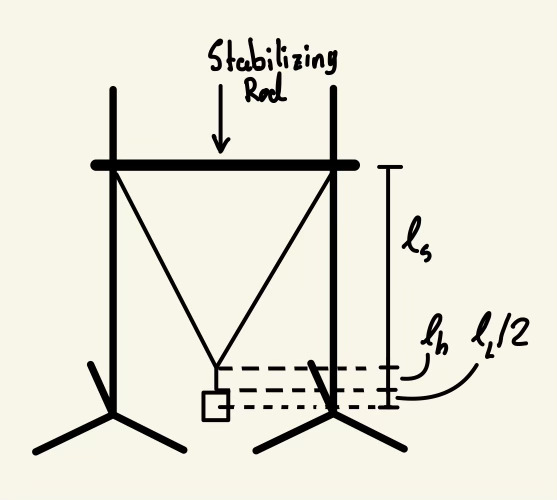
\includegraphics[width=.35\textwidth]{img/side.jpg}
		\caption{Side view of the pendulum apparatus. Included are definitions of the lengths used in center of mass calculations}

	\end{flushright}
\end{wrapfigure}

The goal of the experimental apparatus was to maximize the stability and symmetry of the pendulum with higher masses, and minimize any movement in the direction perpendicular to the plane of motion. Additionally, it must be easy to adjust the string length and mass of the pendulums. A schematic of the final pendulum design is displayed from the front and from the side in \bref{side}{Figure 1} and \bref{front}{Figure 2}.\\


The triangular two pivot design depicted in \bref{front}{Figure 1} was used to solve the problem of the mass oscillating in a direction other than the $\pm \theta$ direction. This was very effective solution, noticeably reducing this motion.\\\\

\begin{wrapfigure}{l}{0.22\textwidth}\label{front}
	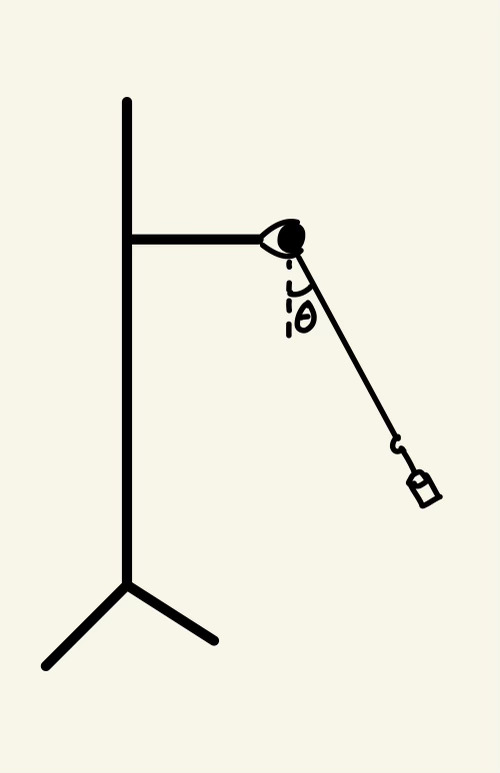
\includegraphics[width=.2\textwidth]{img/front.jpg}
	\caption{Front view of pendulum apparatus}
	\vspace{10pt}
\end{wrapfigure}


To minimize the deflection in the pendulum stand affecting the results, the decision was made to use two stands. Each stand had a clamp that was connected to a metal stabilizing rod. The two clamps were set to the same height and the angle of the stabilizing rod was verified with a level.\\\\


The string that the mass was connected to was run underneath the stabilizing rod, sandwiching it between the rod and the clamps on both sides. This allowed the pivot to not have a clear bias to either side and allowed a simple adjustment for the pendulum length by loosening the clamp and pulling the string through.\\\\

A camera was set up a sufficient distance from the experiment such that it was able to see the mass through all of its motion up to $60^o$. The view from this camera was in the orientation of \bref{front}{Figure 2} and the stabilizing rod was used to align the camera to be perpendicular to the plane of motion.

\subsection{Experimental Procedure}
For every experiment, the vertical length of the pendulum from the axis to the hook was measured (length $\ell_s$ in \bref{front}{Figure 1}). This was done by lowering a string with a mass on the end from the center of the stabilizing rod to get a vertical measurement, aligning this with the hook on the pendulum mass and then measuring the length of that string. Additionally, all angle measurements were done using a protractor that was aligned with the pendulum at rest to get a zero measurement.
\subsubsection{Varying length}
This experiment was performed on three values of $\ell_s$: $(35.5\pm0.1)\unit{cm}, (31.2\pm0.1)\unit{cm},(19.0\pm0.1)\unit{cm}$. In addition to this, each experiment was performed with three initial angles ($\theta_0$): $(15\pm3)^o, (30\pm3)^o,(60\pm3)^o$. The $(200.0\pm 0.1)\unit{g}$ mass was used in this experiment. For each angle/length combination, two trials were filmed in one recording using the camera. In each trial, the pendulum was set to the appropriate length, released from the appropriate angle and allowed to swing for four whole periods. This recording was saved for further analysis.
\subsubsection{Varying release angle}
The $(200.0\pm 0.1)\unit{g}$ mass was used for this experiment and $\ell_s$ was measured as $(30\pm 0.1)\unit{cm}$. This experiment was performed with six initial angles ($\theta_0$): $\pm(15\pm3)^o, \pm(30\pm3)^o,\pm(60\pm3)^o$. For each of these angles, two trials were filmed. The pendulum was set to the appropriate angle and allowed to swing for four whole periods, giving a total of 48 measured periods (8 for each angle).
\subsubsection{Varying mass}
This experiment was performed on four masses: $(20.0\pm0.1)\unit{g},(100.0\pm0.1)\unit{g},(200.0\pm0.1)\unit{g},(500.0\pm0.1)\unit{g},$ and with three initial angles ($\theta_0$): $(15\pm3)^o, (30\pm3)^o,(60\pm3)^o$. Additionally, $\ell_s$ was measured as $(35.5\pm0.1)\unit{cm}$. For each of the mass/angle combinations, the same procedure as the previous two experiments was followed. The mass was released from the appropriate angle with the appropriate mass and two trials of four periods were performed, recording each trial using the camera.
\subsubsection{Measuring Decay}
In this experiment, the pendulum was set up with the $(200.0\pm 0.1)\unit{g}$ mass, released from $(15\pm3)^o$ with a length of $(30.0\pm0.1)\unit{cm}$. In this experiment, the pendulum was allowed to decay until it was approaching zero motion. This process took around 280s and was entirely recorded using the camera.
\subsection{Video analysis}
\subsubsection{Measuring periods}
For the varied length, varied release angle and varied mass experiments, the goal was to measure the period of oscillations. This was done by first using the application `ffmpeg' to overlay a frame count on the video and then using the video player `mpv' to watch the video, using the frame step tool to identify the frame in which the pendulum reached max amplitude. These frames were noted down in a spreadsheet and using the frames per second of the camera ($30\unit{fps}$) this allowed the period of oscillations to be calculated.
\subsubsection{Tracking decay}
To track the decay experiment, the tracker app was used. This is a video analysis and tracking software that provides the ability to track trajectories \cite{tracker}. At the start of the video, the pendulum was left with no energy to create a reference angle of $0^o$. This was used to calibrate the axis and determine the center point of the pendulum. Then using the auto-track feature, this application returned set of $(x,y)$ coordinates with corresponding timestamps that could be used to calculate $\theta(t)$.

\section{Results and Analysis}
\subsection{Periods, lengths and masses}\label{uncertainty}
As mentioned in the methodology section, the periods of each configuration in the varied length, mass and angle experiments were measured in terms of frame number. The camera that was used operates at $t_{fr} = 30\unit{fps}$. If $F_f$ and $F_s$ denote the final and start frames of a period, then the length of the period is then given by: $T = t_{fr}\cdot (F_f-F_s)$. Considering that there is ambiguity in where in the frame the max amplitude was reached, it follows that a half frame uncertainty is a reasonable estimation: $u(F_f)=u(F_s) = 0.5$. Therefore, by \bref{eqn::genUncert}{Equation 5}, it follows that:
\[u(T) = \sqrt{t_f^2\Delta F_f^2 + t_f^2\Delta F_s^2} \approx 0.02\]
This is the uncertainty that was used for all period measurements. The uncertainty of the mass is $0.1\unit{g}$ for all masses and the uncertainty of all length measurements is $0.1\unit{cm}$.
\subsection{Calculating distance to center of mass}\label{sec::distance}
For every measurement, the height of the mass that was used was measured, along with the corresponding hook length (note all of these values are detailed in \bref{side}{Figure 2}). Approximating the center of mass as halfway down the mass and applying \bref{eqn::genUncert}{Equation 5} to the uncertainty gives:
\begin{align*}
	l = \ell_s + \ell_h + \frac{\ell_L}2\pm\sqrt{\ell_s^2 + \ell_h^2 +\left( {\ell_L}/2 \right)}
\end{align*}
For example for a 200g weight with $\ell_h = (3.2\pm 0.1)\unit{cm}$, $\ell_L = (4.5\pm0.1)\unit{cm}$ and for a $(35.5\pm0.1)\unit{cm}$ string length as used in the variable mass experiment, the center of mass distance is given:
\[l = 35.5 + 4.5/2 + 3.2 \pm (\sqrt{(0.1)^2 + (0.1/2)^2 + (0.1^2)}) = (40.95\pm 0.15)\unit{cm}\]
\subsection{Varying Length}
\begin{wrapfigure}{r}{0.4\textwidth}\label{plt::length}
	\vspace{-20pt}
	\centering
		\includegraphics[width=.4\textwidth]{../python/output/variableLength/all.pdf}
		\caption{Plot of measured periods for a pendulum with mass $(200.0\pm0.1)\unit{g}$ vs the length from the pivot to the approximate center of mass. Contains values for initial release angles of $(15\pm 3)^o$, $(30\pm 3)^o$, and $(60\pm 3)^o$. The plot also includes best fit lines for a square root fit for each release angle and one for all values.}
\end{wrapfigure}
By following the procedure described in \bref{uncertainty}{Section 3.1}, the periods for all he samples were calculated. These values were then plotted in \bref{plt::length}{Figure 3}. To verify the effectiveness of the model in \bref{eqn::omegaValue}{Equation 3}, we performed a square root fit of period vs length. Fits were calcualated for the 15, 30 and 60 degree data sets separately, and for all of the data points as well giving four separate fits. Fits were done using the following function in conjunction with the scipy.optimize curve\_fit function. These fits are shown in \bref{plt::length}{Figure 3}. Additionally, plots for each individual release angle are displayed in the appendix.

\begin{lstlisting}[label={func::sqrt}, captionpos=b,language=python]
def sqrt(x, a):
	return a * np.sqrt(x)
\end{lstlisting}

The coefficient $a$ in this scenario is equal to $2\pi  \sqrt g$. This value is approximately equal to $2.006$. The calculated coefficients were $(2.023 \pm 0.009)\unit{s\per\sqrt{m}}$, $(2.045 \pm 0.009)\unit{s\per\sqrt{m}}$ and $(2.096 \pm 0.009)\unit{s\per\sqrt{m}}$ for the 15, 30 and 60 degree release angle data respectively. Although they were all somewhat close to the literature value, there is a clear trend of deviation as the angle increases. This is likely due to the increasing inaccuracy of the small angle approximation at larger angles.\\\\
The fits all had a relatively good fit quality, displaying a $\chi_{red}^2$ of 1.389, 1.446, 1.361 for the 15, 30 and 60 degree plots respectively. The fit for all samples had a noticeably higher chi squared of 1.957, likely due to the deviation in the 60 degree samples not allowing for as tight a fit over the whole data set. Overall, the data suggests that the model that was tested is reasonably accurate, however test with larger angles could perhaps benefit from a more sophisticated model.

\subsection{Varying release angle}
\begin{wrapfigure}{r}{0.4\textwidth}\label{plt::angle}
	\centering
	\vspace{-20pt}
	\includegraphics[width=.55\textwidth]{../python/output/variableAngle/plot.pdf}
	\caption{Plot of measured periods for a pendulum with string length $(35.5\pm 0.1)\unit{cm}$ and mass $(200.0\pm 0.1)\unit{g}$ vs the initial angle of release. The plot also includes a constant best fit of all measured periods.}
\end{wrapfigure}
By following the procedure described in \bref{uncertainty}{Section 3.1}, the periods for all samples were calculated. These values were then plotted in \bref{plt::angle}{Figure 4}. To verify the effectiveness of the model in \bref{eqn::omegaValue}{Equation 3}, a constant fit of period vs angle was performed as there is no angular dependence in this relation. The fit was done using the following function in conjunction with the scipy.optimize curve\_fit function. The fitted graph is displayed in \bref{plt::angle}{Figure 4}.
\begin{lstlisting}[label={func::const}, captionpos=b,language=python]
def constant(x, A):
    return np.full(len(x), A)
\end{lstlisting}
In this part of the experiment, the coefficient $A$ is the period of oscillations. Considering that the pendulum length is $(30.5\pm 0.1)\unit{cm}$ the method described in Section 3.2 can be used to approximate the distance from the pivot to the center of mass. This gives a pendulum length of $(0.353\pm0.002)\unit{m}$. Applying \bref{eqn::omegaValue}{Equation 3} and using \bref{eqn::genUncert}{Equation 5} to propagate error, the theoretical period can be calculated as $(1.195\pm 0.001)\unit{s}$. This is relatively close to the measured value, however there seems to be a non-insignificant difference of approximately 0.02 seconds that is unaccounted for. This could be due to the large angle measurements biasing the result away from the small angle approximation.

\subsection{Varying mass}
\begin{wrapfigure}{r}{0.4\textwidth}\label{plt::mass}
	\centering
	\vspace{-20pt}
		\centering
		\includegraphics[width=.55\textwidth]{../python/output/variableMass/all.pdf}
		\caption{Plot of measured periods for a pendulum with string length $(35.5\pm 0.1)\unit{cm}$ vs the mass at the end of the pendulum. Measurements are made with $\theta_0$ values: $(15\pm 3)^o$, $(30\pm 3)^o$, and $(60\pm 3)^o$. Includes constant fit for all data sets.}

		\vspace{-100pt}
\end{wrapfigure}
By following the procedure described in \bref{uncertainty}{Section 3.1}, the periods for all samples were calculated. These values were then plotted in \bref{plt::mass}{Figure 5}, separated by their initial release angles. To verify the effectiveness of the model in \bref{eqn::omegaValue}{Equation 3}, a constant fit of period vs mass was applied to each group of measurements with the same initial release angle. This was done as there is no mass dependence in the theoretical relation. The fit was done using the same constant function as the last experiment. The fitted graph is displayed in \bref{plt::angle}{Figure 5}.\\\\
In the same manner as the last experiment, the theoretical period for the pendulum was calculated to be $(1.284\pm 0.001)\unit{s}$. There was again a clearly larger value in the fitted period values of $(1.324\pm 0.004)\unit{s}$, $(1.336\pm 0.003)\unit{s}$ and $(1.374\pm 0.003)\unit{s}$ for 15, 30 and 60 degree sample sets respectively. Further investigation is required to determine the source of this increased pendulum period, however it could possibly be due to some form of dissipative force such as air resistance or friction that is not accounted for in this model. This would reduce the average speed of the mass, increasing its period. This is further supported by the low chi squared values of approximately 1 for every data set.

\subsection{Measuring decay}
\begin{figure}[H]\label{decayPlots}
	\centering
	\begin{minipage}[t]{0.45\textwidth}
		\centering
		\includegraphics[width=\textwidth]{../python/output/decay/plot.pdf}
		\caption{Plot of angle from equilibrium position vs time for a simple pendulum left to decay.}
	\end{minipage}
	\hfill
	\begin{minipage}[t]{0.45\textwidth}
		\centering
		\includegraphics[width=\textwidth]{../python/output/decay/envelope.pdf}
		\caption{Plot containing an estimation of the max amplitude at 100 equally spaced points within the oscillation. The max amplitude is estimated as the maximum absolute angle in each 2.8s interval and is placed at the center of this interval. Plot contains best fit for exponential decay. }
	\end{minipage}
\end{figure}
\bref{decayPlots}{Figure 6} displays the raw data that was collected from the tracker application after it had been converted from $(x,y)$ position to angles by applying $\arctan$. The tracking application tended to have issues tracking one specific point of the mass and tended to jump around a lot. Due to this, error in both the $x$ and $y$ measurements from the tracker were set to the diagonal length of the mass's body. This gave an unceratinty of $3cm$. To propagate this uncertainty to the angle that is displayed in the graph, \bref{eqn::genUncert}{Equation 5} was used giving:
\[ u(\theta) = \sqrt{\left({y\over x^2 + y^2}\right)^2u(x)^2 + \left({x\over x^2 + y^2}\right)^2u(y)^2}\]
It appears as if an exponential decay envelope is present, but to verify this theory, further analysis was required. By dividing the data sets into 100 intervals and taking the maximum absolute angle measured in each of these intervals, \bref{decayPlots}{Figure 7} was produced. This plot acts as an approximation of how the decay envelope progressed over time. An exponential decay fit was applied to this model resulting in an extremely low $\chi_{red}^2$ of $0.3350$. This likely suggests that the error was overestimated. The measured $\tau$ value was given as $\tau = (179\pm1)\unit{s}$. Even though the high error seems to have created an ``over fit scenario'', there is still a very clear trend of exponential decay visible in the plot.
\section{Conclusion}
The purpose of this experiment was to provide a comprehensive analysis of the effectiveness of the damped simple pendulum model \bref{eqn::oscillatorEqn}{Equation 1}. Through this study we observed that the model proved to be remarkably accurate. The analysis suggested that the square root relationship between the length and the period was accurate but tended to lose accuracy at higher angles. Similarly, the models of constant period in relation to changes in mass and initial angle proved to be very accurate as well. The damping model of exponential decay seemed to also be extremely accurate in the experimental data. A future study should investigate further how the model deviates at high angles and attempt to determine a more sophisticated model that fits these scenarios more accurately.
\bibliographystyle{apacite}
\bibliography{references.bib}
\end{document}
